\chapter{Exciton Population Statistics in Semiconductor Nanocrystals}    % First appendix chapter, i.e., Appendix A.

\section{Overview}     % This is appendix section 1.
As described in the introductory chapter of this thesis, quantum confinement in semiconductor nanocrystals manifests as a discrete, molecule-like density of states. One consequence of this state quantization is that nanocrystals absorb integral numbers of photons from an applied electromagnetic field. Furthermore, at pump energies in excess of the band gap, rapid intraband thermalization (see Chapter 2) ensures that carrier-induced absorption saturation at the pump wavelength is minimal. As a result, the probability of generating an electron-hole pair in an NC is relatively independent of the number of electron-hole pairs already existing in it. Together, these factors permit modeling of excitations in NC ensembles as discrete random variables, which are well-described by Poissonian statistics. 

\section{Poisson Statistics}  % This is appendix subsection 1.
Originally developed in an effort to model the number of wrongful criminal convictions in a given country \cite{poisson1837probabilite}, the Poisson distribution is a discrete probability distribution which expresses the chance of a given number of events occurring in a fixed interval or time or space, assuming these events occur independently of the time/distance to the previous event. In general, a discrete random variable $X$ is said to exhibit a Poisson distribution if the probability mass function of $X$ is given by:
\begin{equation}\label{eq:poiss1}
f(k; \lambda) = \mathrm{Pr}(X = k) = \frac{\lambda^k}{k!}e^{-\lambda}
\end{equation}
In Eq. \ref{eq:poiss1}, the parameter $\lambda$ is a "success rate", \emph{i.e.} the number of successes in a given interval such that $\lambda = np$, where $n$ is the number of trials and $p$ is the probability of success for each trial.

\subsection{Derivation}  % This is subsubsection 1.
The Poisson distribution is actually a limiting case of a more familiar discrete probability distribution, the binomial distribution. The binomial distribution is given by:
\begin{equation}\label{eq:poiss2}
\mathrm{Pr}(X = k) = \frac{n!}{k!\left(n - k\right)!}p^k(1 - p)^{n - k}
\end{equation}
As noted above, we define $\lambda = np$.  Solving for $p$, we see $p = \lambda/n$. To arrive at the Poisson distribution, we substitute for $p$ and take the limit as the number of trials becomes very large.
\begin{equation}\label{eq:poiss3}
\lim_{n\to\infty} \mathrm{Pr}(X = k) = \lim_{n\to\infty}\frac{n!}{k!\left(n - k\right)!}\left(\frac{\lambda}{n}\right)^k\left(1 - \frac{\lambda}{n}\right)^{n - k}
\end{equation}
Pulling out a common factor of $\lambda^k/k!$, we arrive at Equation \ref{eq:poiss4}:
\begin{equation}\label{eq:poiss4}
\lim_{n\to\infty} \mathrm{Pr}(X = k) = \left(\frac{\lambda^k}{k!}\right) \lim_{n\to\infty} \frac{n!}{\left(n - k\right)!}\left(\frac{1}{n^k}\right)\left(1 - \frac{\lambda}{n}\right)^n\left(1 - \frac{\lambda}{n}\right)^{-k}
\end{equation}
Evaluating each of the terms on the right hand side of Eq. \ref{eq:poiss4} in the limit of large $n$, we get:
\begin{equation}\label{eq:poiss5}
\left(\frac{\lambda^k}{k!}\right) \lim_{n\to\infty} \frac{n!}{\left(n - k\right)!}\left(\frac{1}{n^k}\right)\left(1 - \frac{\lambda}{n}\right)^n\left(1 - \frac{\lambda}{n}\right)^{-k} = \left(\frac{\lambda^k}{k!}\right)\left(1\right)\left(e^{-\lambda}\right)\left(1\right)
\end{equation}
This simplifies to the Poisson distribution:
\begin{equation}\label{eq:poiss6}
f(k; \lambda) = \mathrm{Pr}(X = k) = \frac{\lambda^k}{k!}e^{-\lambda}
\end{equation}
Therefore the Poisson distribution is a special case of the binomial distribution given a very large number of trials.

\subsection{Application to Semiconductor Nanocrystal Absorption}
We may re-cast the Poisson distribution in the form used commonly in the NC literature by defining the success rate $\lambda$ as the average number of photons absorbed per nanocrystal, $\left\langle N_0\right\rangle$, and $k$ as $m$, the number of photogenerated electron-hole pairs per nanocrystal. Then, the probability of having $m$ electron-hole pairs in a particular NC given an average electron-hole population of $\left\langle N_0\right\rangle$ is:
\begin{equation}\label{eq:poissNC1}
P_m = \frac{\left\langle N_0\right\rangle^m}{m!}e^{-\left\langle N_0\right\rangle}
\end{equation}
In Eq. \ref{eq:poissNC1}, $\left\langle N_0\right\rangle$ is known from the experimental pump fluence $j_p$ and the per-nanocrystal absorption cross section, $\sigma_a$; $\left\langle N_0\right\rangle = \sigma_a \cdot j_p$. The Poisson distribution is shown for several values of $\left\langle N_0\right\rangle$ in Figure \ref{f:poisson1} assuming an ensemble of 10$^6$ 4 nm-diameter CdSe nanocrystals.

\begin{figure}
\begin{center}
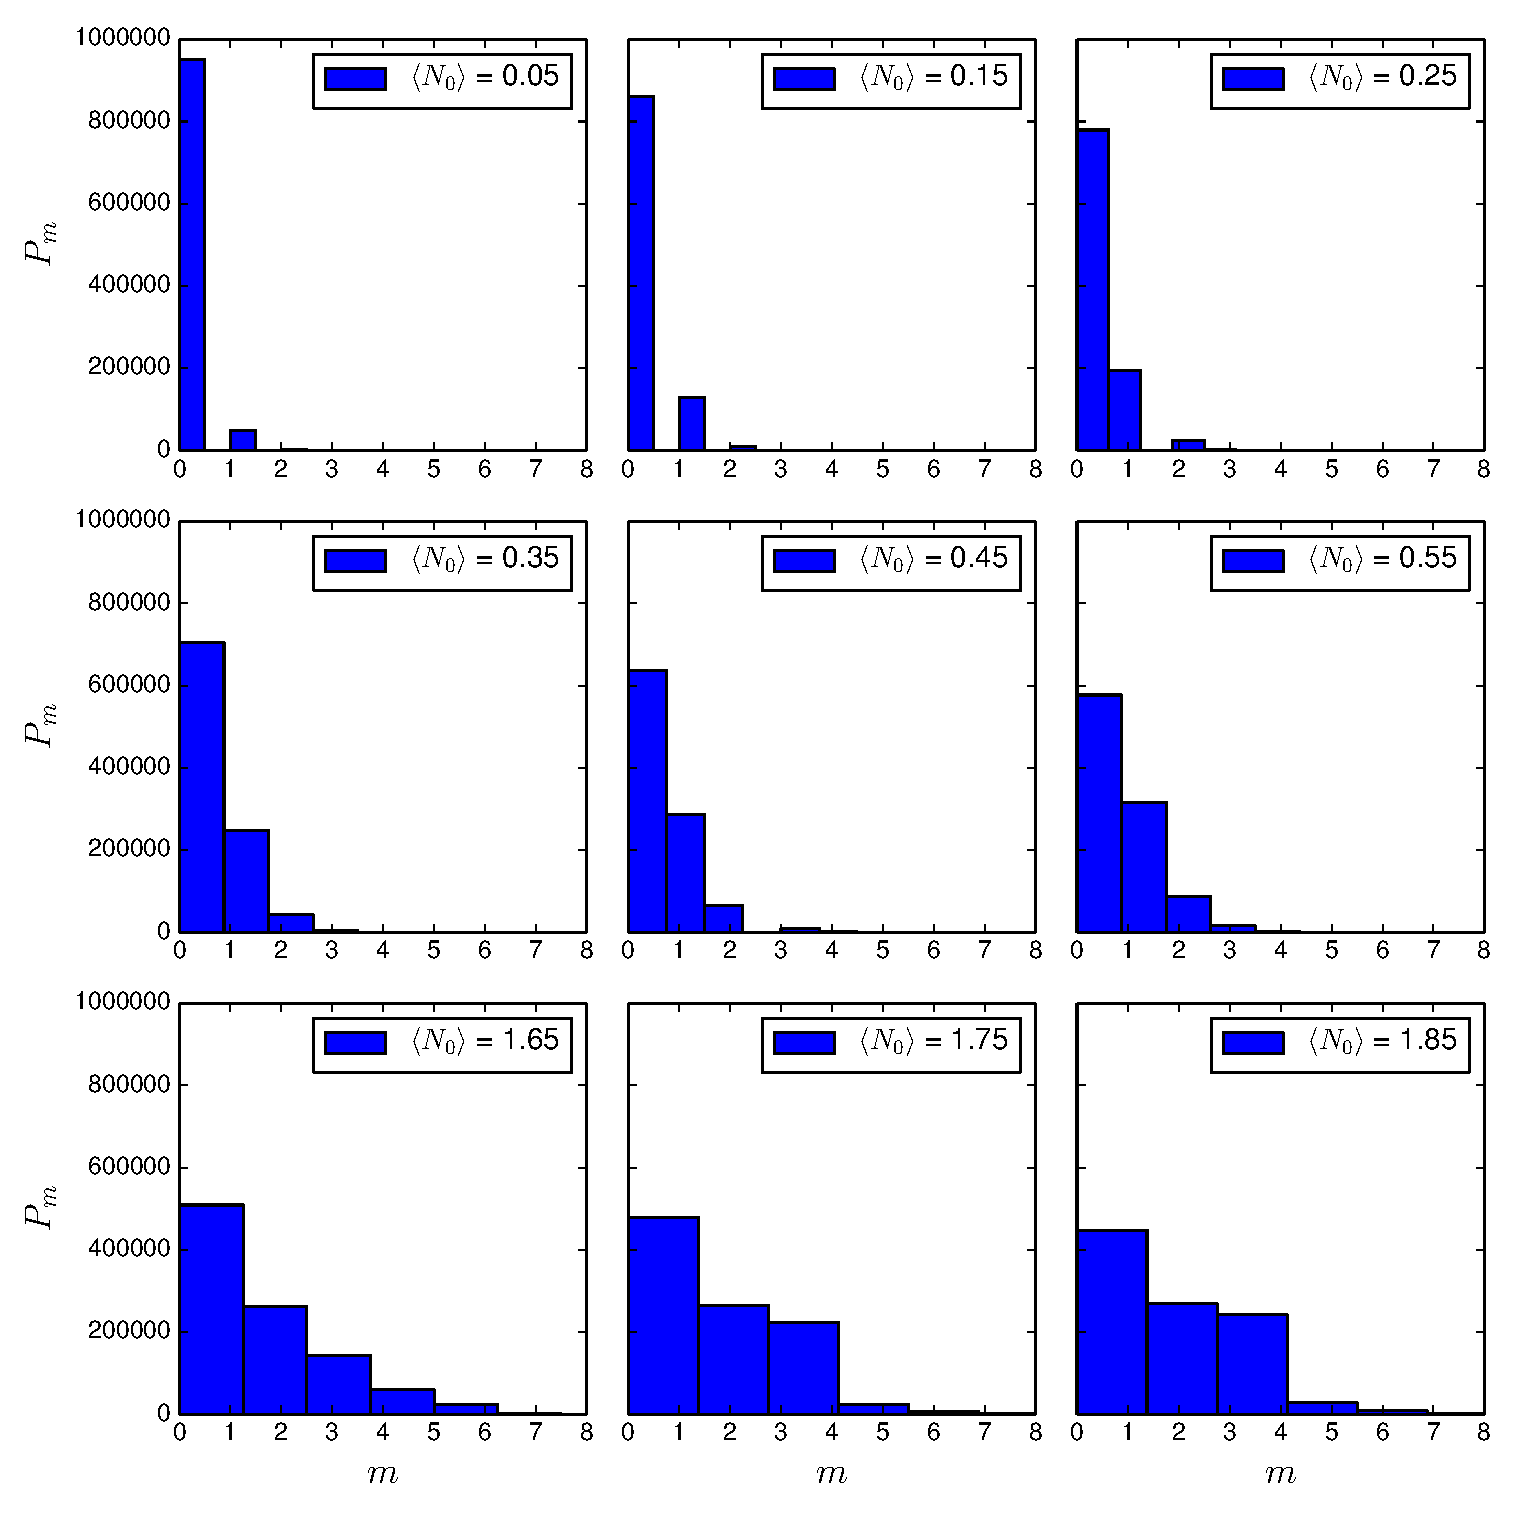
\includegraphics[width=\textwidth]{./appendixA/poisson1.pdf}
\caption[Poisson distribution for nanocrystal exciton populations for various simulated pump fluences.]{Histograms of a Poisson distribution for a variety of $\left\langle N_0\right\rangle$ values, indicated on the figure panels, for an ensemble of 10$^6$ 4 nm-diameter CdSe NCs.}
\label{f:poisson1}
\end{center}
\end{figure}

As is clear from Fig. \ref{f:poisson1}, NC populations absorbing more than $\sim$0.2 photons per nanocrystal exhibit appreciable numbers of NCs having more than one photogenerated electron-hole pair ($m > 1$). In most of the studies carried out during the course of this dissertation work, multi-exciton processes such as Auger recombination would serve to complicate the observed dynamics and would obscure direct observation of intrinsic single-carrier cooling processes such as phonon emission. Therefore, unless otherwise explicitly noted, all time-resolved optical experiments in this thesis utilize a pump fluence sufficiently low to ensure $\left\langle N_0\right\rangle \leq$ 0.2. We test this assumption by confirming that observed (single-exciton) dynamics remain unchanged for fluences $\sim$3$\times$ higher or lower than those utilized in the experiment. An example of this test in shown in the context of time-resolved photoluminescence in Figure \ref{f:poisson2}. 

\begin{figure}
\begin{center}
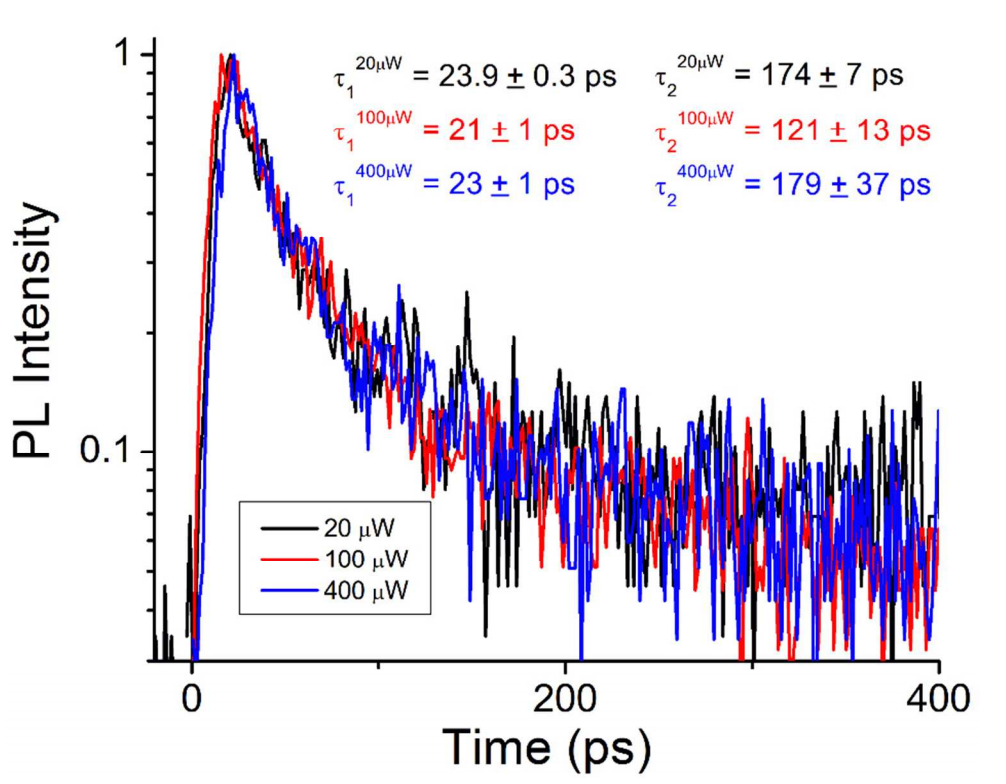
\includegraphics[width=0.65\textwidth]{./appendixA/poisson2.png}
\caption[Time-resolved photoluminescence decay of 3.2 nm-diameter CdSe NCs at 3.6 K at various pump fluences.]{Time-resolved photoluminescence measured at 2.6 K for a 3.2 nm-diameter CdSe NC sample dissolved in solid octadecane. Changes in pump fluence from 20 $\mu$W to 400 $\mu$W at 3 eV using a 2 kHz repitition rate and a 450 micron diameter spot did not produce significant changes in the decay time constants.}
\label{f:poisson2}
\end{center}
\end{figure}

